\documentclass[]{beamer}
\usetheme[shownavsym]{AAUsimple}
\usepackage{lmodern}
\usefonttheme{structurebold} %%%%%%%%%%%%%%%%%%%%%%%%%%%%%%%%%%
\usepackage[utf8]{inputenc}
\usepackage[dutch]{babel}
\usepackage[T1]{fontenc}
\usepackage{tikz}
\tikzset{>=stealth}
\usepackage{microtype}
\usepackage{mathtools}
\usepackage{siunitx}
%%%%%%%%%%%%%%%%%%%%%%%%%%%%%%%%%%
% Gekleurde hyperlinks
\newcommand{\chref}[2]{%
	\href{#1}{{\usebeamercolor[bg]{AAUsidebar}#2}}%
}
\title[Respiratie]{Mechanisme van ventilatie}

\date{\today}

\author[Edon Namani, et. al]
{%
	Edon Namani\\
	\href{mailto:e.namani@student.rug.nl}{{\tt e.namani@student.rug.nl}}
}

\institute[%
	Faculteit Gezondheidswetenschappen\\
	Rijksuniversiteit Groningen\\
	Nederland
]
{%
	Faculteit Gezondheidswetenschappen\\
	Rijksuniversiteit Groningen\\
	Nederland

}

\pgfdeclareimage[height=1.5cm]{titlepagelogo}{AAUgraphics/semper_invicta.pdf}
\titlegraphic{%
	\pgfuseimage{titlepagelogo}
}

\begin{document}
% Titel
{\aauwavesbg%
	\begin{frame}[plain,noframenumbering]
	\titlepage
\end{frame}}
%%%%%%%%%%%%%%%

%TOC
\begin{frame}{Agenda}{}
	\tableofcontents
\end{frame}
%%%%%%%%%%%%%%%
\section{Principes van luchtstroom}
\begin{frame}{Principes van luchtstroom}
    \begin{block}{Ideale gaswet}
        Als de hoeveelheid mol gas en temperatuur gelijk blijft, dan geldt voor een druk- en/of volume verandering in een afgesloten ruimte:
            \begin{equation*}
                P_1V_1 = P_2V_2
            \end{equation*}
    \end{block}
    %%%
    \begin{block}{Stroomrichting van lucht}
        Lucht stroomt altijd van een hogedrukgebied naar lagedrukgebied.
    \end{block}
\end{frame}
%%%%%%%%%%%%%%%%%%%%%%%%%%%%%%%%%%
\subsection{Principes toegepast op de long}
\begin{frame}{Principes van luchtstroom}{Toepassing op long}
    \begin{columns}
        \column{.55\textwidth}
        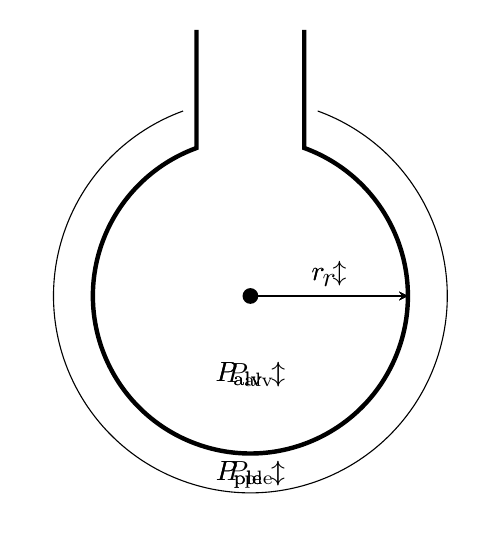
\begin{tikzpicture}
%        \draw (0,0) grid (4,4);
%		\foreach \y in {1,2,...,4}
%		\draw (1mm,\y) -- (-1mm,\y) node[anchor=east] {\y};
%		\foreach \x in {1,2,...,3}
%        \draw (\x,1mm) -- (\x,-1mm) node[anchor=north] {\x};
        \coordinate (C) at (2,2);
        \draw[ultra thick] (C) + (70:2) coordinate (A) 
            (A)  +(0,1.5) coordinate (B) 
            (B) -- (A) arc[start angle=70, end angle=-250, radius=2] -- +(0,1.5);
        \draw (C) +(70:2.5) arc[start angle=70, end angle=-250, radius=2.5]; 
        \onslide<1>{\draw[->] (C) -- (4,2) node[midway, anchor=south] {$r$};}
            \onslide<2-4>{\draw[->] (C) -- (4,2) node[midway, anchor=south] {$r\uparrow$};}
            \onslide<5>{\draw[->] (C) -- (4,2) node[midway, anchor=south] {$r\downarrow$};}
        \fill (C) circle[radius=1mm];
        \onslide<1>{\node at (2,1) {$P_{\text{alv}}$}
            node at (2,-.27) {$P_{\text{ple}}$}    
            ;
    }
    \onslide<2-4>{\node at (2,1) {$P_{\text{alv}}\downarrow$}
                    node at (2,-.27) {$P_{\text{ple}}\downarrow$}
                                ;
                        }
                    \onslide<5>{\node at (2,1) {$P_{\text{alv}}\uparrow$}
                                                    node at (2,-.27) {$P_{\text{ple}}\uparrow$}
                                                                                    ;
                                                                                                        }
    \end{tikzpicture}
        \column{.45\textwidth}
        \begin{enumerate}
            \item<1-> Contractie van ademhalingsspieren
            \item<2-> Daling $P_{\text{ple}}$
            \item<3-> Stijging $V_{\text{alv}}$ $\rightarrow$ daling $P_{\text{alv}}$
            \item<4-> Luchtdrukverschil tussen alveoli en atmosfeer doet lucht naar binnenstromen
            \item<5-> De elasticiteit van thorax en longen maakt $P_{\text{alv}} > P_{\text{atm}}$ 
        \end{enumerate}
    \end{columns}
\end{frame}
%%%%%%%%%%%%%%%%%%%%%%%%%%%%%%%%%%
\section{Compliantie}
\begin{frame}{Compliantie}{Definitie}
    \begin{block}{Definitie pulmonale compliantie}
        Compliantie ($C$) is een maat waarmee de volume van long verandert, als een druk op de long werkt. Mathematisch gedefinieerd:
        \begin{equation*}
            C = \frac{\Delta V}{\Delta P_{\text{transpulmonaal}}}
        \end{equation*}
        Compliantie is de inverse van elasticiteit. Elasticiteit geeft aan hoeveel druk je moet uitvoeren om een volumeverandering van de long te krijgen:
        \begin{equation*}
            E = C^{-1}
        \end{equation*}
        Een hoge compliantie betekent een lage elasticiteit en vice versa.
\end{block}
\end{frame}
\subsection{Factoren van compliantie}
\begin{frame}{Compliantie}{Factoren}
    \begin{block}{Compliantie verlagende factoren}
    \begin{itemize}
        \item Elasticiteit
            \begin{itemize}
                \item Ribbenkast, e.g. kyfoscoliose
                \item Longen $\rightarrow$ elastine, collageen, oppervlaktespanning water
            \end{itemize}
        \item Wrijving
            \begin{itemize}
                \item Luchtweerstand
                \item Weefselweerstand
            \end{itemize}
    \end{itemize}
    \end{block}
\end{frame}
\subsection{$PV$-curve}
    \begin{frame}{Compliantie}{$PV$-curve}
\begin{columns}
    \column{.62\textwidth}
    \only<1>{%
    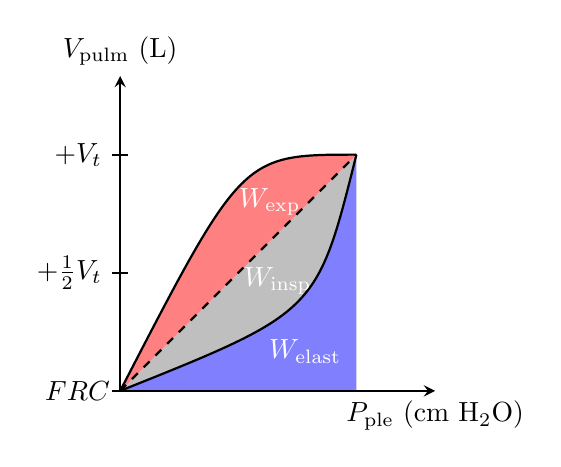
\begin{tikzpicture}[thick]
                \coordinate (A) at (3,3);
               %\draw (0,0) grid (4,4);
               %\foreach \y in {1,2,...,4}
               %\draw (1mm,\y) -- (-1mm,\y) node[anchor=east] {\y};
               %\foreach \x in {1,2,...,3}
               % \draw (\x,1mm) -- (\x,-1mm) node[anchor=north] {\x};
                \fill[fill=blue!50] (0,0) -- (A) -- +(0,-3) -- cycle;
                \draw (1mm,3) -- (-1mm,3) node [anchor=east] {$+V_t$}
                    (1mm,1.5) -- (-1mm,1.5) node[anchor=east] {$+\frac{1}{2}V_t$}
                    (-1mm,0) -- (0,0) node[anchor=east] {$FRC$};
                \draw[<->]  (0,4) -- (0,0) -- (4,0) node[anchor=north] {$P_{\text{ple}}$ (\si{\centi\meter} H\textsubscript{2}O)};
                \node[anchor=south] at (0,4) {$V_{\text{pulm}}$ (\si{\litre})};
                \draw[fill=gray!50!] (0,0) .. controls (2.5,1) .. (A);
                \draw[fill=red!50!] (0,0) .. controls (1.55,3) .. (A);
                \draw[dashed] (0,0) -- (3,3) ;
                \node[white] at (1.9,2.40) {$W_{\text{exp}}$}
                    node[white] at (2,1.4) {$W_{\text{insp}}$}
                node[white] at (2.35,.5) {$W_{\text{elast}}$};
                %\draw (0,0) (A) .. controls + (-140:.5) and +(40:5.31) .. (0,0);
    \end{tikzpicture}
}
\only<2>{%
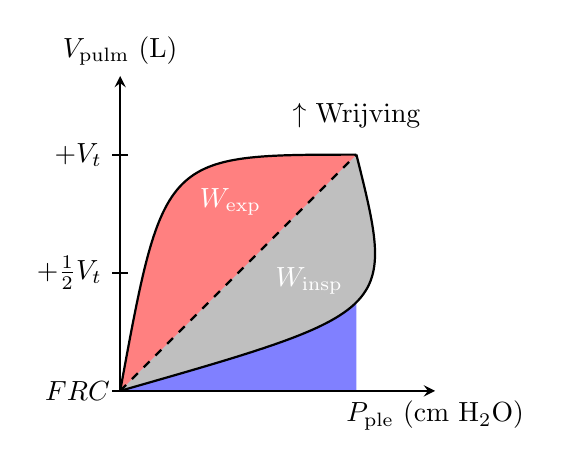
\begin{tikzpicture}[thick]
                \coordinate (A) at (3,3);
               %\draw (0,0) grid (4,4);
               %\foreach \y in {1,2,...,4}
               %\draw (1mm,\y) -- (-1mm,\y) node[anchor=east] {\y};
               %\foreach \x in {1,2,...,3}
               % \draw (\x,1mm) -- (\x,-1mm) node[anchor=north] {\x};
                \fill[fill=blue!50] (0,0) -- (A) -- +(0,-3) -- cycle;
                \draw (1mm,3) -- (-1mm,3) node [anchor=east] {$+V_t$}
                    (1mm,1.5) -- (-1mm,1.5) node[anchor=east] {$+\frac{1}{2}V_t$}
                    (-1mm,0) -- (0,0) node[anchor=east] {$FRC$};
                \draw[<->]  (0,4) -- (0,0) -- (4,0) node[anchor=north] {$P_{\text{ple}}$ (\si{\centi\meter} H\textsubscript{2}O)};
                \node[anchor=south] at (0,4) {$V_{\text{pulm}}$ (\si{\litre})};
                \draw[fill=gray!50!] (0,0) .. controls (3.5,1) .. (A);
                \draw[fill=red!50!] (0,0) .. controls (0.55,3) .. (A);
                \draw[dashed] (0,0) -- (3,3) ;
                \node[white] at (1.4,2.40) {$W_{\text{exp}}$}
                    node[white] at (2.4,1.4) {$W_{\text{insp}}$};
                \node at (3,3.5) {$\uparrow$ Wrijving};
                %\draw (0,0) (A) .. controls + (-140:.5) and +(40:5.31) .. (0,0);
    \end{tikzpicture}
}
\column{.38\textwidth}
    \begin{itemize}
        \item De compliantie is de raaklijn aan de curve
        \item De ademarbeid is de oppervlakte onder de curve
        \item $\uparrow$ wrijving $\rightarrow$ breder grafiek
        \item Verandering in elasticiteit doet alleen de grafiek roteren, strekken of krimpen.
    \end{itemize}
\end{columns}
\end{frame}
\subsection{Maatregelen van lichaam tegen de factoren}
\begin{frame}{Compliantie}{Maatregelen van lichaam tegen de factoren}
    \begin{block}{Surfactant}
        Type II alveolicellen produceren surfactant, fosfolipiden. Fosfolipiden verbreken de water-lucht interface door hun amfifiele eigenschap $\rightarrow$ Daling oppervlaktespanning $\rightarrow$ Stijging compliantie.
    \end{block}
    %%%
    \begin{block}{Luchtwegverwijderaars}
        Het lichaam heeft hormonen, zoals adrenaline, die doen aan bronchodilatatie. Een verhoogd $P_\text{CO\textsubscript{2}}$ heeft hetzelfde effect. Bronchodilatatie vermindert luchtweerstand.
    \end{block}
\end{frame}
%%%%%%%%%%%%%%%%%%%%%%%%%%%%%%%%%%
\section{Spirogram}
\begin{frame}{Spirogram}
    \begin{columns}
        \column{.65\textwidth}
    \begin{tikzpicture}[thick]
        \usebeamercolor{frametitle}
               \draw[<->] (0,6.3) -- ++(0,-5.8) -- ++(5,0) node[anchor=west] {$t$};
               \foreach[count=\y] \V in {1000,2000,...,6000}{%
                   \draw (1mm,\y) -- (-1mm,\y) node[anchor=east] {\V};
           }
           \node[anchor=south] at (0,6.3) {$V$ (\si{\milli\litre})};
           \draw[bg] (0,2.3) .. controls (.25,2.3) and (.25,2.8) .. (.5,2.8)
                    .. controls (.75,2.8) and (.75,2.3) .. (1,2.3)
                    .. controls (1.25,2.3) and (1.25,2.8) .. (1.5,2.8) 
                    .. controls (1.75,2.8) and (1.75,2.3) .. (2,2.3)
                    .. controls (2.25,2.3) and (2.25,5.8) .. (2.5,5.8)
                    .. controls (2.75,5.8) and (2.75,1.2) .. (3,1.2)
                    .. controls (3.25,1.2) and (3.25,2.8) .. (3.5,2.8)
                    ;
                \begin{scope}[every node/.style={white}]
                    \fill[blue!60] (3.75,.5) rectangle (4.75,5.8);
                    \node at (4.25,4.3) {$V_{ir}$}
                        node at (4.25,2.55) {$V_t$} 
                        node at (4.25,1.75) {$V_{er}$}
                        node at (4.25,.8) {$V_r$}
                    ;
                \end{scope}
                \draw[<->] (5.1,5.8) -- node[fill=white,inner sep=2]{VC} +(0,-4.6);
                \draw[<->](5.6,.4) -- node[fill=white,inner sep=2]{FRC} +(0,1.9);
                \draw[dashed,black] (0,2.3) -- +(5,0)
                              (0,2.8) -- +(5,0) 
                              (0,1.2) -- +(5,0)
                              (0,5.8) -- +(5,0)
                    ;
    \end{tikzpicture}
    \column{.35\textwidth}
    Bij restrictieve en obstructieve longziektes wijken de volumes af.
\end{columns}
\end{frame}
%%%%%%%%%%%%%%%%%%%%%%%%%%%%%%%%%%
\section{Dode ruimte}
\begin{frame}{Dode ruimte}
    \begin{block}{Definitie}
        Dode ruimte is ruimte waarin ingeademde lucht zit die niet deelneemt aan gaswisseling. Er zijn twee varianten van dode ruimte:
        \begin{enumerate}
            \item Anatomisch dode ruimte, e.g. trachea, bronchiën
            \item Fysiologische dode ruimte, lucht in de respiratoire zone van longen waar geen perfusie is
        \end{enumerate}
    \end{block}
\end{frame}
{\aauwavesbg
\begin{frame}[plain,noframenumbering]
	\finalpage{Voor het ``Oh ja! Ik wist dat!'' gevoel!}
\end{frame}}
\end{document}
